\documentclass[tikz,border=5pt]{standalone}
\usepackage[T1]{fontenc}
\usepackage{lmodern,amsmath,amssymb}
\usetikzlibrary{arrows.meta,calc,positioning,fit,backgrounds,shapes.geometric,matrix,decorations.pathreplacing,patterns}
\definecolor{ink}{gray}{0.08}
\definecolor{wash}{gray}{0.965}
\definecolor{soft}{gray}{0.45}
\tikzset{box/.style={draw=ink,line width=.65pt,fill=white,align=center,inner sep=4pt,outer sep=0pt,font=\small},flow/.style={draw=ink,line width=.65pt,-{Latex[length=1.8mm,width=1.3mm]},rounded corners=2pt},annotation/.style={font=\scriptsize,text=soft,align=center},groupbox/.style={draw=soft,dashed,line width=.45pt,fill=wash}}
\begin{document}
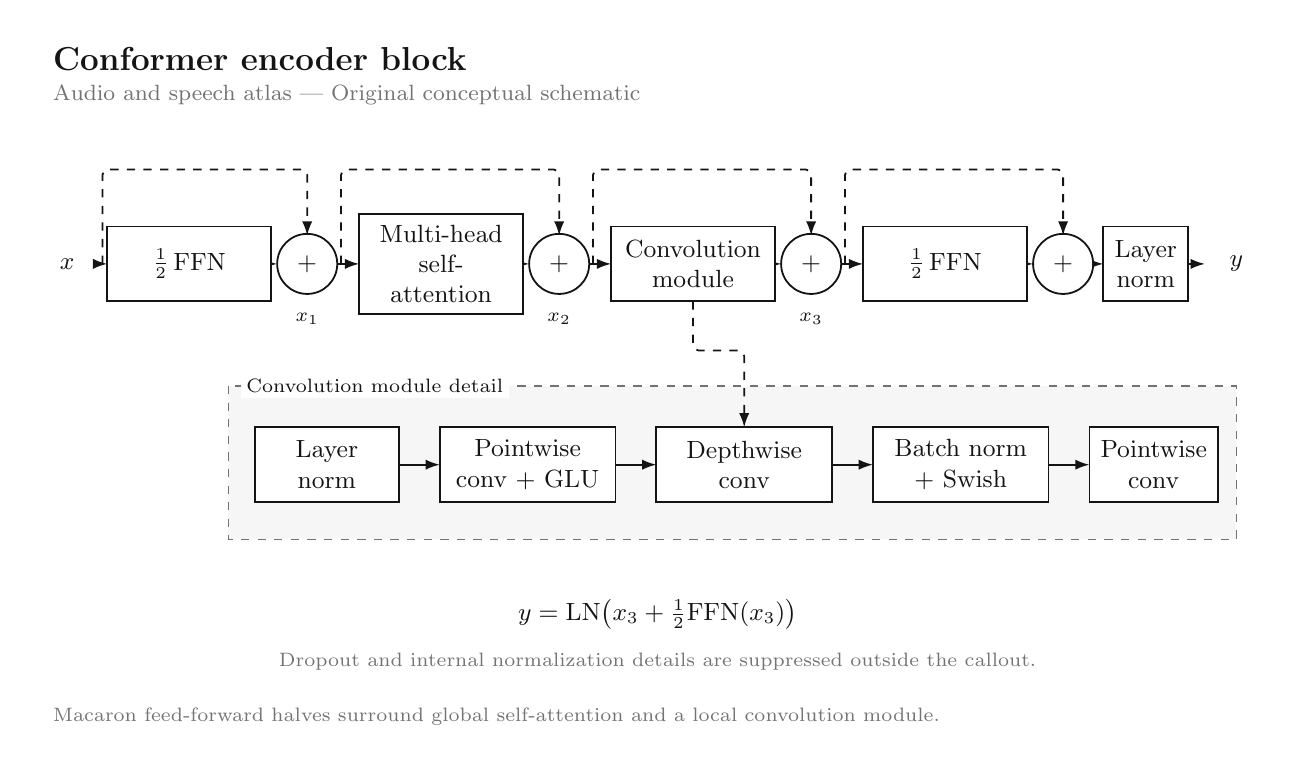
\begin{tikzpicture}[x=1cm,y=-1cm,font=\rmfamily,text=ink]

\path[use as bounding box] (0,0) rectangle (16,9);
\node[anchor=west,font=\large\bfseries] at (.2,.4) {Conformer encoder block};
\node[anchor=west,font=\footnotesize,text=soft] at (.2,.85) {Audio and speech atlas | Original conceptual schematic};
\begin{pgfonlayer}{background}
\draw[groupbox] (2.55,4.55) rectangle (15.350000000000001,6.5);
\node[anchor=west,font=\scriptsize,fill=white,inner sep=2pt] at (2.6999999999999997,4.55) {Convolution module detail};
\end{pgfonlayer}
\node[align=center,inner sep=0pt,outer sep=0pt,font=\small,minimum width=0.8cm,minimum height=0.65cm,text width=0.55cm] (input) at (0.5,3.0) {$x$};
\node[box,minimum width=2.05cm,minimum height=0.95cm,text width=1.7999999999999998cm] (ff1) at (2.05,3.0) {$\tfrac12\,\mathrm{FFN}$};
\node[box,circle,minimum width=0.55cm,minimum height=0.55cm,text width=0.30000000000000004cm] (ff1sum) at (3.55,3.0) {$+$};
\node[box,minimum width=2.05cm,minimum height=0.95cm,text width=1.7999999999999998cm] (mhsa) at (5.25,3.0) {Multi-head\\self-attention};
\node[box,circle,minimum width=0.55cm,minimum height=0.55cm,text width=0.30000000000000004cm] (mhsasum) at (6.75,3.0) {$+$};
\node[box,minimum width=2.05cm,minimum height=0.95cm,text width=1.7999999999999998cm] (conv) at (8.45,3.0) {Convolution\\module};
\node[box,circle,minimum width=0.55cm,minimum height=0.55cm,text width=0.30000000000000004cm] (convsum) at (9.95,3.0) {$+$};
\node[box,minimum width=2.05cm,minimum height=0.95cm,text width=1.7999999999999998cm] (ff2) at (11.65,3.0) {$\tfrac12\,\mathrm{FFN}$};
\node[box,circle,minimum width=0.55cm,minimum height=0.55cm,text width=0.30000000000000004cm] (ff2sum) at (13.15,3.0) {$+$};
\node[box,minimum width=1.05cm,minimum height=0.95cm,text width=0.8cm] (ln) at (14.2,3.0) {Layer\\norm};
\node[align=center,inner sep=0pt,outer sep=0pt,font=\small,minimum width=0.8cm,minimum height=0.65cm,text width=0.55cm] (out) at (15.35,3.0) {$y$};
\node[box,minimum width=1.8cm,minimum height=0.95cm,text width=1.55cm] (cln) at (3.8,5.55) {Layer norm};
\node[box,minimum width=2.2cm,minimum height=0.95cm,text width=1.9500000000000002cm] (glu) at (6.35,5.55) {Pointwise\\conv + GLU};
\node[box,minimum width=2.2cm,minimum height=0.95cm,text width=1.9500000000000002cm] (dw) at (9.1,5.55) {Depthwise\\conv};
\node[box,minimum width=2.2cm,minimum height=0.95cm,text width=1.9500000000000002cm] (bn) at (11.85,5.55) {Batch norm\\+ Swish};
\node[box,minimum width=1.6cm,minimum height=0.95cm,text width=1.35cm] (pw) at (14.3,5.55) {Pointwise\\conv};
\begin{pgfonlayer}{background}
\draw[flow] (input.east) -- (ff1.west);
\draw[flow] (ff1.east) -- (ff1sum.west);
\draw[flow] (ff1sum.east) -- (mhsa.west);
\draw[flow] (mhsa.east) -- (mhsasum.west);
\draw[flow] (mhsasum.east) -- (conv.west);
\draw[flow] (conv.east) -- (convsum.west);
\draw[flow] (convsum.east) -- (ff2.west);
\draw[flow] (ff2.east) -- (ff2sum.west);
\draw[flow] (ff2sum.east) -- (ln.west);
\draw[flow] (ln.east) -- (out.west);
\draw[flow] (cln.east) -- (glu.west);
\draw[flow] (glu.east) -- (dw.west);
\draw[flow] (dw.east) -- (bn.west);
\draw[flow] (bn.east) -- (pw.west);
\draw[flow,dashed] (conv.south) -- (8.45,4.1) -- (9.1,4.1) -- (dw.north);
\end{pgfonlayer}
\draw[flow,dashed] (0.95,3.0) -- (0.95,1.8) -- (3.55,1.8) -- (3.55,2.64);
\draw[flow,dashed] (3.98,3.0) -- (3.98,1.8) -- (6.75,1.8) -- (6.75,2.64);
\draw[flow,dashed] (7.18,3.0) -- (7.18,1.8) -- (9.95,1.8) -- (9.95,2.64);
\draw[flow,dashed] (10.379999999999999,3.0) -- (10.379999999999999,1.8) -- (13.15,1.8) -- (13.15,2.64);
\node[align=center,anchor=center,font=\scriptsize,text=ink,text width=1cm] at (3.55,3.7) {\mbox{$x_1$}};
\node[align=center,anchor=center,font=\scriptsize,text=ink,text width=1cm] at (6.75,3.7) {\mbox{$x_2$}};
\node[align=center,anchor=center,font=\scriptsize,text=ink,text width=1cm] at (9.95,3.7) {\mbox{$x_3$}};
\node[align=center,anchor=center,font=\small,text=ink,text width=12cm] at (8,7.45) {\mbox{$y=\mathrm{LN}\!\left(x_3+\tfrac12\mathrm{FFN}(x_3)\right)$}};
\node[align=center,anchor=center,font=\scriptsize,text=soft,text width=13cm] at (8,8.05) {Dropout and internal normalization details are suppressed outside the callout.};
\node[anchor=west,align=left,font=\scriptsize,text=soft,text width=15.6cm] at (.2,8.75) {Macaron feed-forward halves surround global self-attention and a local convolution module.};
\end{tikzpicture}
\end{document}
